% Also note that the "draftcls" or "draftclsnofoot", not "draft", option
% should be used if it is desired that the figures are to be displayed in
% draft mode.
%

%\documentclass[conference]{IEEEtran}
\documentclass{acm_proc_article-sp}

% correct bad hyphenation here
\hyphenation{op-tical net-works semi-conduc-tor}

% Optionally save space in lists (place this command after a list environment (e.g., itemize, enumerate, description)
\newcommand{\compresslist}{
	\vspace{-1em}
	\setlength{\itemsep}{1pt}
	\setlength{\parskip}{0pt}
	\setlength{\parsep}{0pt}
}


\usepackage{cite}
\usepackage{url}
\usepackage[table, svgnames]{xcolor} 
\usepackage{color}
\usepackage{siunitx}
\usepackage{multirow}
\usepackage{times}
\usepackage{graphicx}
\usepackage{epsf}
\usepackage{verbatim}
\usepackage{psfig}
\usepackage{cite}
\usepackage{url}
\usepackage{color}
\usepackage[table]{xcolor}
\usepackage{booktabs, dcolumn}
\usepackage{alltt}

\usepackage{longtable,lscape}
\usepackage{slashbox,multirow}
\usepackage{colortbl}
\usepackage{mathrsfs}

\newcommand{\Add}{\CodeIn{add}}
\newcommand{\AVTree}{\CodeIn{AVTree}}
\newcommand{\Assignment}[3]{$\langle$ \Object{#1}, \Object{#2}, \Object{#3} $\rangle$}
\newcommand{\BinaryTreeRemove}{\CodeIn{BinaryTree\_remove}}
\newcommand{\BinaryTree}{\CodeIn{BinaryTree}}
\newcommand{\Caption}{\caption}
\newcommand{\Char}[1]{`#1'}
\newcommand{\CheckRep}{\CodeIn{checkRep}}
\newcommand{\ClassC}{\CodeIn{C}}
\newcommand{\CodeIn}[1]{{\small\texttt{#1}}}
\newcommand{\CodeOutSize}{\scriptsize}
\newcommand{\Comment}[1]{}
\newcommand{\Ensures}{\CodeIn{ensures}}
\newcommand{\ExtractMax}{\CodeIn{extractMax}}
\newcommand{\FAL}{field-ordering}
\newcommand{\FALs}{field-orderings}
\newcommand{\Fact}{observation}
\newcommand{\Get}{\CodeIn{get}}
\newcommand{\HashSet}{\CodeIn{HashSet}}
\newcommand{\HeapArray}{\CodeIn{HeapArray}}
\newcommand{\Intro}[1]{\emph{#1}}
\newcommand{\Invariant}{\CodeIn{invariant}}
\newcommand{\JUC}{\CodeIn{java.\-util.\-Collections}}
\newcommand{\JUS}{\CodeIn{java.\-util.\-Set}}
\newcommand{\JUTM}{\CodeIn{java.\-util.\-TreeMap}}
\newcommand{\JUTS}{\CodeIn{java.\-util.\-TreeSet}}
\newcommand{\JUV}{\CodeIn{java.\-util.\-Vector}}
\newcommand{\JMLPlusJUnit}{JML+JUnit}
\newcommand{\Korat}{Korat}
\newcommand{\Left}{\CodeIn{left}}
\newcommand{\Lookup}{\CodeIn{lookup}}
\newcommand{\MethM}{\CodeIn{m}}
\newcommand{\Node}[1]{\CodeIn{N}$_#1$}
\newcommand{\Null}{\CodeIn{null}}
\newcommand{\Object}[1]{\CodeIn{o}\ensuremath{_#1}}
\newcommand{\PostM}{\MethM$_{post}$}
\newcommand{\PreM}{\MethM$_{pre}$}
\newcommand{\Put}{\CodeIn{put}}
\newcommand{\Remove}{\CodeIn{remove}}
\newcommand{\RepOk}{\CodeIn{repOk}}
\newcommand{\Requires}{\CodeIn{requires}}
\newcommand{\Reverse}{\CodeIn{reverse}}
\newcommand{\Right}{\CodeIn{right}}
\newcommand{\Root}{\CodeIn{root}}
\newcommand{\Set}{\CodeIn{set}}
\newcommand{\State}[1]{2^{#1}}
\newcommand{\TestEra}{TestEra}
\newcommand{\TreeMap}{\CodeIn{TreeMap}}

\newenvironment{CodeOut}{\begin{scriptsize}}{\end{scriptsize}}
\newenvironment{SmallOut}{\begin{small}}{\end{small}}

\newcommand{\pairwiseEquals}{PairwiseEquals}
\newcommand{\monitorEquals}{MonitorEquals}
%\newcommand{\monitorWField}{WholeStateW}
\newcommand{\traverseField}{WholeState}
\newcommand{\monitorSMSeq}{ModifyingSeq}
\newcommand{\monitorSeq}{WholeSeq}

\newcommand{\IntStack}{\CodeIn{IntStack}}
\newcommand{\UBStack}{\CodeIn{UBStack}}
\newcommand{\BSet}{\CodeIn{BSet}}
\newcommand{\BBag}{\CodeIn{BBag}}
\newcommand{\ShoppingCart}{\CodeIn{ShoppingCart}}
\newcommand{\BankAccount}{\CodeIn{BankAccount}}
\newcommand{\BinarySearchTree}{\CodeIn{BinarySearchTree}}
\newcommand{\LinkedList}{\CodeIn{LinkedList}}

\newcommand{\Book}{\CodeIn{Book}}
\newcommand{\Library}{\CodeIn{Library}}

\newcommand{\Jtest}{Jtest}
\newcommand{\JCrasher}{JCrasher}
\newcommand{\Daikon}{Daikon}
\newcommand{\JUnit}{JUnit}

\newcommand{\trie}{trie}

\newcommand{\Perl}{Perl}


\newcommand{\SubjectCount}{11}
\newcommand{\DSSubjectCount}{two}

\newcommand{\Equals}{\CodeIn{equals}}
\newcommand{\Pairwise}{PairwiseEquals}
\newcommand{\Subgraph}{MonitorEquals}
\newcommand{\Concrete}{WholeState}
\newcommand{\ModSeq}{ModifyingSeq}
\newcommand{\Seq}{WholeSeq}
\newcommand{\Aeq}{equality}

\newcommand{\Meaning}[1]{\ensuremath{[\![}#1\ensuremath{]\!]}}
\newcommand{\Pair}[2]{\ensuremath{\langle #1, #2 \rangle}}
\newcommand{\Triple}[3]{\ensuremath{\langle #1, #2, #3 \rangle}}
\newcommand{\SetSuch}[2]{\ensuremath{\{ #1 | #2 \}}}

\newcommand{\Equiv}[2]{\ensuremath{#1 \EquivSTRel{} #2}}
\newcommand{\EquivME}{\Equiv}
\newcommand{\EquivST}{\Equiv}
\newcommand{\EquivSTRel}{\ensuremath{\cong}}
\newcommand{\Redundant}[2]{\ensuremath{#1 \lhd #2}}
\newcommand{\VB}{\ensuremath{\mid}}
\newcommand{\MES}{method-entry state}

\newcommand{\Small}[1]{{\small{#1}}}

\newcommand{\CenterCell}[1]{\multicolumn{1}{c|}{#1}}

% Yoonki's code
\colorlet{tableheadcolor}{gray!25} % Table header colour = 25% gray
\newcommand{\headcol}{\rowcolor{tableheadcolor}} %
\colorlet{tablerowcolor}{gray!10} % Table row separator colour = 10% gray
\newcommand{\rowcol}{\rowcolor{tablerowcolor}} %
    % Command \topline consists of a (slightly modified) \toprule followed by a \heavyrule rule of colour tableheadcolor (hence, 2 separate rules)
\newcommand{\topline}{\arrayrulecolor{black}\specialrule{0.1em}{\abovetopsep}{0pt}%
            \arrayrulecolor{tableheadcolor}\specialrule{\belowrulesep}{0pt}{0pt}%
            \arrayrulecolor{black}}
    % Command \midline consists of 3 rules (top colour tableheadcolor, middle colour black, bottom colour white)
\newcommand{\midline}{\arrayrulecolor{tableheadcolor}\specialrule{\aboverulesep}{0pt}{0pt}%
            \arrayrulecolor{black}\specialrule{\lightrulewidth}{0pt}{0pt}%
            \arrayrulecolor{white}\specialrule{\belowrulesep}{0pt}{0pt}%
            \arrayrulecolor{black}}
    % Command \rowmidlinecw consists of 3 rules (top colour tablerowcolor, middle colour black, bottom colour white)
\newcommand{\rowmidlinecw}{\arrayrulecolor{tablerowcolor}\specialrule{\aboverulesep}{0pt}{0pt}%
            \arrayrulecolor{black}\specialrule{\lightrulewidth}{0pt}{0pt}%
            \arrayrulecolor{white}\specialrule{\belowrulesep}{0pt}{0pt}%
            \arrayrulecolor{black}}
    % Command \rowmidlinewc consists of 3 rules (top colour white, middle colour black, bottom colour tablerowcolor)
\newcommand{\rowmidlinewc}{\arrayrulecolor{white}\specialrule{\aboverulesep}{0pt}{0pt}%
            \arrayrulecolor{black}\specialrule{\lightrulewidth}{0pt}{0pt}%
            \arrayrulecolor{tablerowcolor}\specialrule{\belowrulesep}{0pt}{0pt}%
            \arrayrulecolor{black}}
    % Command \rowmidlinew consists of 1 white rule
\newcommand{\rowmidlinew}{\arrayrulecolor{white}\specialrule{\aboverulesep}{0pt}{0pt}%
            \arrayrulecolor{black}}
    % Command \rowmidlinec consists of 1 tablerowcolor rule
\newcommand{\rowmidlinec}{\arrayrulecolor{tablerowcolor}\specialrule{\aboverulesep}{0pt}{0pt}%
            \arrayrulecolor{black}}
    % Command \bottomline consists of 2 rules (top colour
\newcommand{\bottomline}{\arrayrulecolor{white}\specialrule{\aboverulesep}{0pt}{0pt}%
            \arrayrulecolor{black}\specialrule{\heavyrulewidth}{0pt}{\belowbottomsep}}%
\newcommand{\bottomlinec}{\arrayrulecolor{tablerowcolor}\specialrule{\aboverulesep}{0pt}{0pt}%
            \arrayrulecolor{black}\specialrule{\heavyrulewidth}{0pt}{\belowbottomsep}}%

\usepackage{dcolumn}
\newcolumntype{Y}{D..{6.4}}

%\newcommand{\blind}[1]{{\color{white}\{#1\}}}
\newcommand{\blind}[1]{#1}


%
% paper title
% can use linebreaks \\ within to get better formatting as desired
% Do not put math or special symbols in the title.
\begin{document}
\title{Questions Developers Ask While Diagnosing Potential Security Vulnerabilities With Static Analysis}
% What Questions Do Developers Ask When Reasoning about the Security of Their Code? Building Tools that Answer Developers' Questions about Security Vulnerabilities?

\numberofauthors{2}
\author{
\alignauthor Justin Smith, Brittany Johnson, and Emerson Murphy-Hill\\
\affaddr{North Carolina State University}\\
\affaddr{Raleigh, NC 27606} \\
\email{}
\alignauthor Bill Chu and Heather Richter Lipford\\
\affaddr{University of North Carolina at Charlotte}\\
\affaddr{Charlotte, NC 28223}\\
\email{}
%\blind{\{billchu, heather.lipford\}@uncc.edu}
}

\maketitle


% As a general rule, do not put math, special symbols or citations
% in the abstract
\begin{abstract}

Static analysis tools help developers answer questions about potential security vulnerabilities in their code. 
A better understanding of the types of questions asked by developers might help toolsmiths design more effective tools.
Currently, we lack a categorization of such questions. 
We began constructing this categorization by conducting a laboratory experiment with novice and experienced software developers, observing their interactions with security vulnerabilities in iTrust, a Java medical records software system.
The questions participants asked suggest that developers may lack adequate tool support.
In particular, participants employed error-prone strategies while navigating from malicious data sources to sensitive data sinks and while managing all the tasks required to reason about a vulnerability. 

\end{abstract}
% no keywords


\section{Introduction}

Software developers are a critical part of making software secure, a particularly important task considering security vulnerabilities are likely to cause incidents that affect company profits as well as end users~\cite{chen2002mops}.
When software systems contain security defects, often developers must determine the best ways to remove them. 

To assist developers with the task of detecting and removing security defects, toolsmiths provide a variety of static analysis tools.
One of example of such a tool is Find Security Bugs (FSB),\footnote{\url{h3xstream.github.io/find-sec-bugs/}} an extension of FindBugs.\footnote{\url{findbugs.sourceforge.net}} 
FSB locates and reports on potential security vulnerabilities in software, such as SQL injection and cross-site scripting.  
Other tools, such as CodeSonar\footnote{\url{grammatech.com/codesonar}} and Coverity,\footnote{\url{coverity.com/}} can also be used to detect and remove potential security vulnerabilities.
Unfortunately, however, research suggests that developers are not using static analysis tools, in part because tools do not always effectively communicate relevant information to developers~\cite{johnson2013don}. 

% maybe connect back to example.

Although existing work has categorized developers' information requirements in a broad sense, including the notion that developers have questions about the security of their code~\cite{latoza2010hard}, no prior study has specifically investigated questions that developers ask when using tools to diagnose and fix security vulnerabilities. 
As we show later in this paper, many questions are unique to using security tools.

Furthermore, in non-security domains, work that identifies questions has helped toolsmiths improve the state-of-the-art of program analysis tools~\cite{kononenko2012automatically, servant2012history, yoon2013visualization}. Similarly, we expect that categorizing the questions developers ask when using security-focused static analysis tools will help improve those tools and yield better adoption. 


%Though not the goal of their work, many researchers have taken the findings of LaToza and colleagues and been able to work towards improving the state-of-the-art for program analysis tools~\cite{kononenko2012automatically, servant2012history, yoon2013visualization}. 



In this paper, we report a study conducted to create a better understanding of the information developers seek when using static analysis tools to identify and assess security vulnerabilities in code.
We conducted a laboratory experiment with ten developers familiar with the iTrust software system.\footnote{\blind{\url{http://agile.csc.ncsu.edu/iTrust/wiki/doku.php?id=start}}} 
We observed each developer as they assessed potential security vulnerabilities identified by FSB. 
We report the kinds of questions they asked while doing so, along with the strategies they used to answer them.
Using a card sort methodology, we sorted the 559 questions into 17 categories. 

Our work makes three contributions. 
First, we present a categorization of questions software developers ask when fixing security vulnerabilities using a static analysis tool.
Second, based on our observations, we discuss the strategies developers use to answer their questions.
Finally, we evaluate the existing tool support for answering security-related questions.


%Figure, high res, png or vector (pdf)

\section{Related Work}
\label{sec:rw}

We have organized the related work into two subsections. Section \ref{evaluation} outlines the predominant approaches researchers use to evaluate security tools and Section \ref{questions} references similar studies that have explored the questions developers ask when modifying, understanding, or debugging their code.

\subsection{Evaluation of Techniques}
\label{evaluation}
Developers use several techniques and tools to help secure their systems.
Using a variety of metrics, many studies have assessed the effectiveness of the tools and techniques developers use to find and remove vulnerabilities from their code~\cite{martin2005finding, austin2011one, livshits2005finding}.  

Much research has evaluated the effectiveness of tools and techniques based on their false positive rates and how many vulnerabilities they detect~\cite{jovanovic2006pixy, austin2011one, dukes2013case}. 
Jovanovic and colleagues attempt to address the problem of vulnerabilities in web applications by implementing and evaluating \textsc{Pixy}, a static analysis tool that detects cross-site scripting vulnerabilities in PHP scripts~\cite{jovanovic2006pixy}. 
They considered their tool effective because of its low false positive rate (50\%) and its ability to find vulnerabilities previously unknown. 
Similarly, Livshits and Lam evaluated their own approach to static analysis for detecting security vulnerabilities; the static analyzers used are created from specifications provided by the user~\cite{livshits2005finding}. 
They also found their tool to be effective because it had a low false positive rate. 

Austin and Williams compared the effectiveness of four existing techniques for discovering security vulnerabilities: systematic and exploratory manual  penetration testing, static analysis, and automated penetration testing~\cite{austin2011one}. 
Comparing the four approaches based on number of vulnerabilities found, false positive rate, and efficiency, they reported that no one technique was capable of discovering every type of vulnerability. 
Dukes and colleagues conducted a case study comparing static analysis and manual testing techniques used to find security vulnerabilities~\cite{dukes2013case}. 
They found combining manual testing and static analysis was most effective, because it located the most vulnerabilities.


These studies use various measures of effectiveness, such as false positive rates or vulnerabilities found by a tool, but none focus on how developers interact with the tool. 
Further, they do not evaluate whether the tools under study answer questions developers have about the code or vulnerabilities. 

\subsection{Answering Developer Questions}
\label{questions}
Several studies have explored the knowledge requirements of developers when coding.
Similar to our work, some existing studies focus on the questions developers ask to determine these knowledge requirements~\cite{latoza2010hard, latoza2010developers}.
In contrast, our study focuses specifically on the knowledge requirements of developers when assessing security vulnerabilities.


Much of the work on answering developer questions has occurred in the last decade. 
LaToza and Myers surveyed professional software developers to understand the questions developers ask during their daily coding activities, focusing on the hard to answer questions~\cite{latoza2010hard}. 
Futhermore, after observing developers in a lab study, they discovered that the questions developers ask tend to be questions revolving around searching through the code for target statements, or reachability questions~\cite{latoza2010developers}. 
Ko and Myers developed \textsc{Whyline}, a tool meant to ease the process of debugging code by helping answer ``why did'' and ``why didn't'' questions~\cite{ko2004designing}. 
They found that developers were able to complete more debugging tasks when using their tool than they could without it.
Fritz and Murphy developed a model and prototype tool to assist developers with answering the questions they want to ask based on interviews they conducted~\cite{fritz2010using}.

Our work builds on the work of LaToza and Myers, which found that some of the hard-to-answer questions developers have surround the implications of code changes on the security of their code. 

\section{Methodology}
\label{sec:meth}
We conducted a laboratory experiment with ten software developers. In our analysis, we extracted and categorized the questions developers asked during each study session. 
Section \ref{rqs} outlines the research questions we sought to answer. 
Section \ref{studyDesign} details how the study was designed and Section \ref{dataAnalysis} describes how we performed data analysis.
Experimental materials can be found online.\footnote{\blind{\url{http://www4.ncsu.edu/~bijohnso/security-questions.html}}}


\subsection{Research Questions}
\label{rqs}
We want to answer the following research questions:
\begin{itemize}
\compresslist
\item \textbf{RQ1}: What types of security related questions do developers ask?
\item \textbf{RQ2}: How do current tools and approaches support developers in answering these questions?
\end{itemize}


\subsection{Study Design}
\label{studyDesign}
Each session started with a five-minute briefing section, which included time for participants to familiarize themselves with the study environment and Find Security Bugs (FSB).
Following the briefing period, participants progressed through encounters with four vulnerabilities. 
Figure \ref{fig:environment} depicts the configuration of the integrated development environment (IDE) for one of these encounters.
All participants consented to participate in our study, which had institutional review board approval, and to have their session recorded using screen and audio capture software.
Finally, each session concluded with several demographic and open-ended discussion questions.

\begin{figure}
	\centering
	\includegraphics[width=3.5in]{Images/environment.png}
	\caption{The study environment.}
	\label{fig:environment} 
\end{figure}



\subsubsection{Materials}
Participants used Eclipse to explore vulnerabilities in iTrust, an open source Java medical records web application that ensures the privacy and security of patient records according to the HIPAA statute.\footnote{\url{hhs.gov/ocr/privacy/}} 
During the briefing session, participants were given time to familiarize themselves with the development environment and ask any questions about the experimental setup.
Participants were equipped with a version of FindBugs extended with FSB.
We chose FSB because of its low barriers to adoption; it is free, open source, easy to install and configure, and contained within the integrated development environment (IDE). FSB is also similar to other more sophisticated static analysis tools --- such as those listed by NIST,\footnote{\url{samate.nist.gov/index.php/Source_Code_Security_Analyzers.html}} OWASP,\footnote{\url{owasp.org/index.php/Source_Code_Analysis_Tools}} and WASC\footnote{\url{projects.webappsec.org/w/page/61622133/StaticCodeAnalysisList}} --- in terms of the types of security vulnerabilities it detects.



\begin{table}
\centering
\caption{Demographics of study participants}
\begin{tabular}{|l|l|c|S|}
\rowcolor{gray!50}
\hline
    Participant		& Job Title 						& Vulnerability 			&\multicolumn{1}{c|}{Experience} \\
    \rowcolor{gray!50}
    				&									& Familiarity				&   \multicolumn{1}{c|}{Years} \\
    \hline
    P1			    & Student     						& \raisebox{-0.9ex}{
\includegraphics[height=9px]{images/two-half-stars.pdf}} 	&  4.5    \\
    \hline
    P2			    & Test Engineer    					& \raisebox{-0.9ex}{
\includegraphics[height=9px]{images/three-stars.pdf}}		&  8 		\\
    \hline
    P3 				& Development Tester       			& \raisebox{-0.9ex}{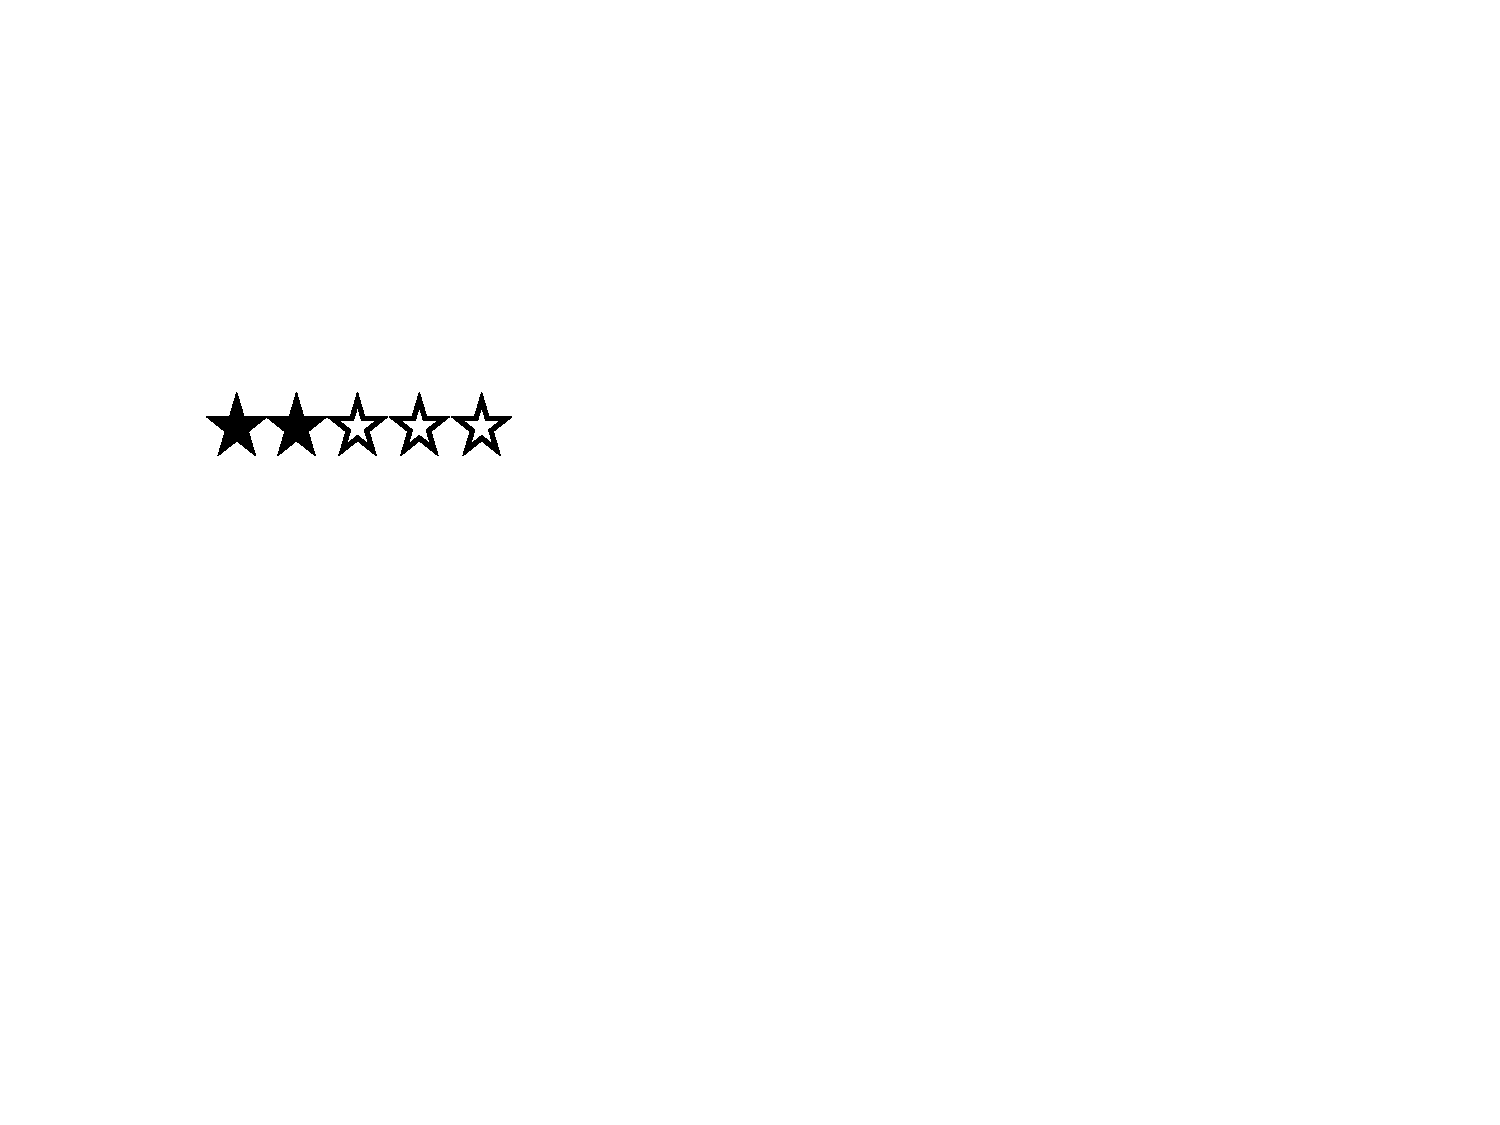
\includegraphics[height=9px]{images/two-stars.pdf}}			&  6 	    	\\
    \hline
    P4				& Software Developer     			& \raisebox{-0.9ex}{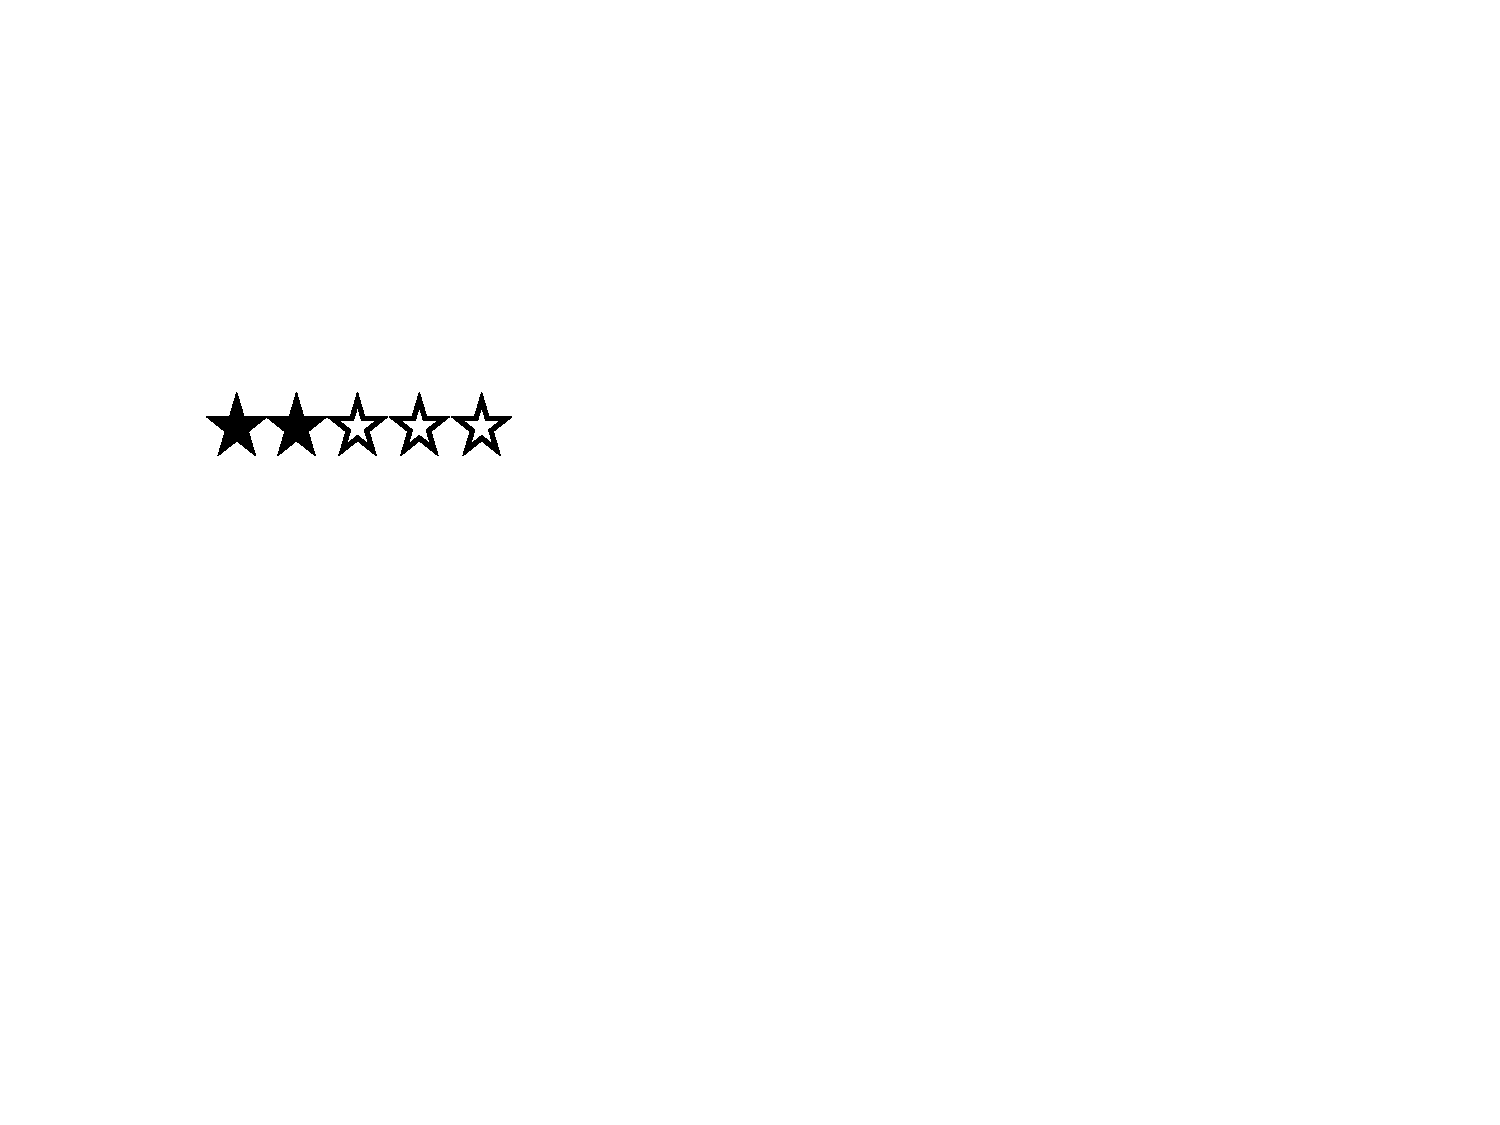
\includegraphics[height=9px]{images/two-stars.pdf}}			&  6     	\\
    \hline
    P5				& Student      						& \raisebox{-0.9ex}{
\includegraphics[height=9px]{images/four-stars.pdf}}			&  10 	\\
    \hline
    P6				& Student		    				& \raisebox{-0.9ex}{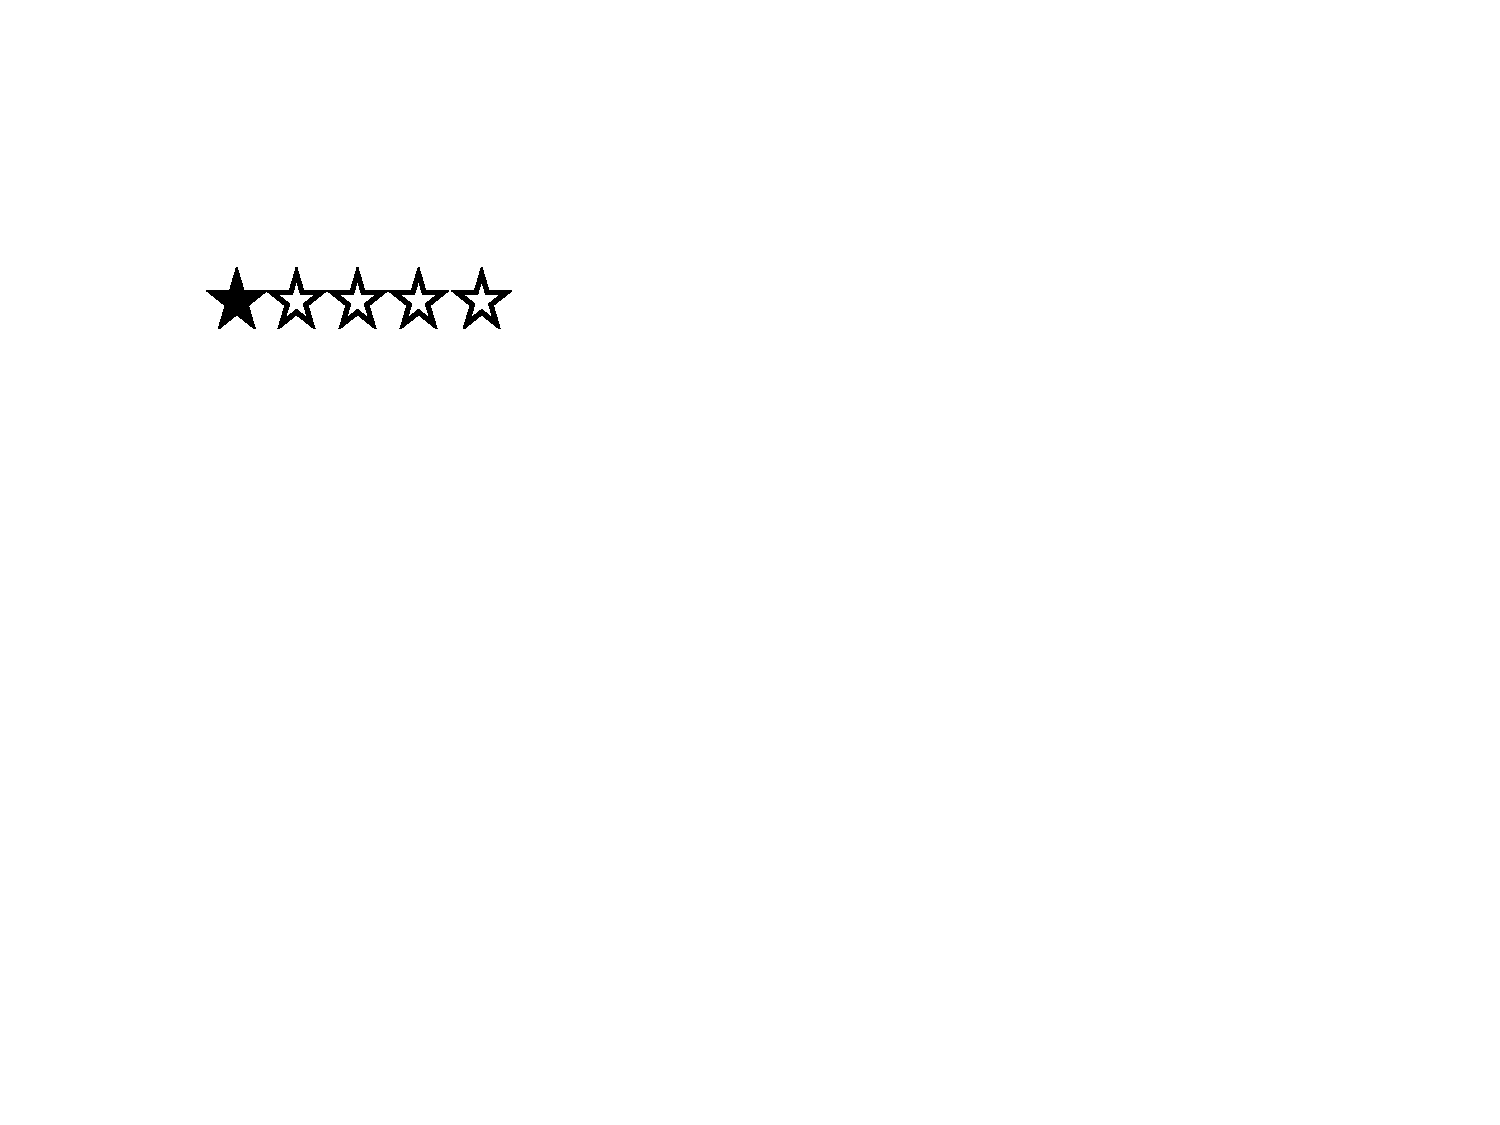
\includegraphics[height=8.5px]{images/one-star.pdf}}				& 4		\\
    \hline
    P7				& Software Developer    	& \raisebox{-0.9ex}{
\includegraphics[height=9px]{images/four-stars.pdf}}		& 4.5         \\
    \hline
    P8				& Student	    					& \raisebox{-0.9ex}{
\includegraphics[height=9px]{images/three-stars.pdf}}		& 7   \\
    \hline
    P9				& Software Consultant   	 		& \raisebox{-0.9ex}{
\includegraphics[height=9px]{images/three-stars.pdf}}		& 5	  		 \\
    \hline
    P10			    & Student    						& \raisebox{-0.9ex}{
\includegraphics[height=9px]{images/three-stars.pdf}}		& 8	           \\
    \hline
\end{tabular}
\label{table:participants}
\end{table}



\subsubsection{Participants}

To simulate a realistic work environment, participants were required to have significant experience working on the iTrust code base. 
All participants either completed or served as teaching assistants for a semester-long software engineering course that focused on developing iTrust.

For our experiment, we recruited ten software developers, five students and five professionals. Participants ranged in programming experience from 4 years to 10 years, averaging 6.3 years.
All sessions were conducted in-person.
We recruited participants from personal contacts and class rosters, using snowball sampling to find additional qualified participants.
Since extracting data from each session required intensive analysis, we ceased recruitment when we determined that we had reached saturation~\cite{glaser2009discovery} and few new questions were emerging from each additional session.

Table~\ref{table:participants} gives additional demographic information on each of the ten participants. 
Participants self-reported their familiarity with security vulnerabilities on a 5 point Likert scale.
In the remainder of this paper, we will refer to participants by the abbreviations found in the participant column of the table.  
Since the focus of our study is to identify the questions developers ask independent of their background, we report on experience to ensure a degree of diversity in our sample and contextualize participants' responses.

\subsubsection{Tasks}
Each participant was asked to assess four vulnerabilities. 
We presented each participant with this number of vulnerabilities, because in preliminary pilot sessions, participants spent approximately 10-15 minutes with each vulnerability and showed signs of fatigue after 60 minutes.

When selecting tasks, we gave preference to existing iTrust vulnerabilities.
To give participants the opportunity to ask as many different types of questions as possible, we ensured each vulnerability was categorized differently by FSB.
Without modifying iTrust, FSB identified vulnerabilities from three different topics: cross-site scripting, path traversal, and predictable random vulnerabilities.
To include a fourth topic, we added a SQL injection vulnerability to iTrust by making minimal alterations to one of the database access objects.
Our modification preserved the functionality of the original code and was based on examples of SQL injection found on OWASP and in open-source projects.
Table \ref{table:vulnerabilities} summarizes each of the four vulnerabilities. 

\begin{table*} 
\centering
\caption{Four vulnerability exploration tasks}
\begin{tabular}{|l|l|l|}
\rowcolor{gray!50}
\hline
    Vulnerability				& Short Description													& Severity Rank 	\\
    \hline	
    Potential Path Traversal	& An instance of java.io.File is created to read a file.     			& ``Scary''	    \\
    \hline
    Predictable Random			& Use of java.util.Random is predictable. 								& ``Scary''		\\
    \hline
    Servlet Parameter 			& The method getParameter returns a String value that is controlled by the client.			& ``Troubling''	\\
    \hline
    SQL Injection				& [Method name] passes a non-constant String to an execute method on an SQL statement.     	& ``Of Concern'' \\
    \hline
\end{tabular}
\label{table:vulnerabilities}
\end{table*}

During the briefing section, we asked participants to pretend they are in charge of security for iTrust and to approach the vulnerabilities as if they were in their normal work environment.
Additionally, we asked them to use a think-aloud protocol, which encourages the participant to verbalize their thought process as they complete a task or activity~\cite{nielsen2002getting}. 
Specifically, they were asked to, ``Say any questions or thoughts that cross your mind regardless of how relevant you think they are.''
We recorded both audio and the screen as experimental artifacts for data analysis.


\subsection{Data Analysis}
\label{dataAnalysis}
We analyzed session data using an approach inspired by grounded theory~\cite{glaser2009discovery}. 
First, we transcribed all the audio-video files using oTranscribe.\footnote{\url{otranscribe.com}}
Each transcript, along with the associated recording, was analyzed by two of the authors for implicit and explicit questions. 
The two question sets for each session were then iteratively compared against each other until the authors reached agreement on the question sets. 
In the remainder of this section, we will detail the question extraction process and question sorting processes, including the criteria used to determine which statements qualified as questions.
\subsubsection{Question Criteria}
Participants ask both explicit and implicit questions. 
Drawing from previous work on utterance interpretation~\cite{letovsky1987cognitive}, we developed five criteria to assist in the uniform classification of participant statements. 
A statement was coded as a question only if it met one of the following criteria:

\begin{itemize}
\compresslist	
\item \textbf{The participant explicitly asks a question.}
\\ Example: \textit{Why aren't they using \CodeIn{PreparedStatements}?}
\item \textbf{The participant makes a statement and explores the validity of that statement.}
\\ Example: \textit{It doesn't seem to have shown what I was looking for. Oh, wait! It's right above it...}
\item \textbf{The participant uses key words such as, ``I assume,'' ``I guess,'' or ``I don't know.''}
\\ Example: \textit{I don't know that it's a problem yet.}
\item \textbf{The participant clearly expresses uncertainty over a statement.}
\\ Example: \textit{Well, it's private to this object, right?}
\item \textbf{The participant clearly expresses a knowledge requirement by describing plans to acquire information.}
\\ Example: \textit{I would figure out where it is being called.}

\end{itemize}

\subsubsection{Question Extraction}
Using the criteria outlined in the previous section, two of the authors independently coded each session. 
When we identified an explicit question or implicit question, which is a statement that satisfies one or more of the criteria, we marked the transcript, highlighted the participant's original statement, and clarified the question being asked.
Question clarification typically entailed rewording the question to best reflect the information the participant is trying to acquire.
From the ten sessions, the first coder extracted 421 question statements; the other coder extracted 389. 

To make sure our categorization of questions was exhaustive, two independent reviewers coded the transcripts using the criteria.
It was sometimes difficult to determine what statements should be extracted as questions; the criteria helped ensure both reviewers only highlighted the statements that reflected actual questions. 


\subsubsection{Question Review}
To remove duplicates and ensure the validity of all the questions, each transcript was reviewed jointly by the two authors that initially coded it.
During the second pass, the two reviewers examined each question statement, discussing the justification for each question based on the previously stated criteria.
The two reviewers merged duplicate questions, favoring the wording that was most strongly grounded in the experiment artifacts.
This process resulted in a total of 559 questions.

Each question that was only identified by one author required verification.
If the other author did not agree that such a question met at least one of the criteria, the question was removed from the question set and counted as a disagreement.
The reviewers were said to agree when they merged a duplicate or verified a question. Depending on the participant, inter-reviewer agreement ranged from 91\% to 100\%. Across all participants, agreement averaged to 95\%.
The agreement scores suggest that the two reviewers consistently held similar interpretations of the question criteria.

\subsubsection{Question Sorting}
To organize our questions and facilitate discussion, we performed an \textit{open} card sort~\cite{hudson2013sorting}. 
Card sorting is typically used to help structure data by grouping related information into categories. 
In an \textit{open} sort, the sorting process begins with no notion of predefined categories. 
Rather, sorters derive categories from emergent themes in the cards. 

We performed our card sort in three distinct stages: clustering, categorization, and validation.
In the first stage, we formed question clusters by grouping questions that identified the same information requirements. 
In this phase we focused on rephrasing similar questions and grouping duplicates.
For example, P1 asked, \textit{Where can I find information related to this vulnerability?} P7 asked, \textit{Where can I find an example of using \CodeIn{PreparedStatements}?} and P2 asked, \textit{Where can I get more information on path traversal?} 
Of these questions, we created a question cluster labeled \textit{Where can I get more information?}
At this stage, we discarded five unclear or non pertinent questions and organized the remaining 554 into 155 unique question clusters.

\begin{table*} 
\centering
\caption{Organizational Groups and Emergent Categories}
\begin{tabular}{|l|l|r|c|}
\rowcolor{gray!50}
\hline
    Group											& Category										& Clusters		& Location in Paper	  	\\
    \hline			
    \multirow{4}{*}{Vulnerabilities, Attacks, and Fixes}
        											& Understanding Alternative Fixes and Approaches	& 11     		& Section~\ref{uafa}	\\

    												& Preventing and Understanding Potential Attacks	& 11     		& Section~\ref{pupa}		\\

    												& Assessing the Application of the Fix				& 9     		& Section~\ref{aaf}				\\

    												& Relationship Between Vulnerabilities							& 3     		& Section~\ref{rbb}			\\
    \hline
    \multirow{4}{*}{Code and the Application}	
    												& Locating Information 								& 11      		& Section~\ref{li}		\\

    												& Control Flow and Call Information					& 13     		& Section~\ref{cf}	\\

    												& Data Storage and Flow								& 11     		& Section~\ref{dsf}  	\\

    												& Code Background and Functionality	 				& 17     		& Section~\ref{cbf}			\\

    									& Application Context/Usage										& 9     		& Section~\ref{acu}			\\

    									& End-User Interaction											& 3     		& Section~\ref{eui}		\\
    \hline	
    \multirow{4}{*}{Individuals}	
    									& Developer Planning and Self-Reflection						& 14    		& Section~\ref{dpr}		\\

    									& Understanding Concepts										& 6 			& Section~\ref{uc}			\\

    									& Confirming Expectations					 					& 1				& Section~\ref{ce}  \\
    \hline
	\multirow{4}{*}{Problem Solving Support}

    									& Vulnerability Severity and Rank											& 4     		& Section~\ref{bsr}		\\

    									& Understanding and Interacting with Tools						& 9     		& Section~\ref{uit}			\\

   	 									& Resources and Documentation									& 10     		& Section~\ref{rd}		\\

    									& Notification Text												& 3     		& Section~\ref{em}		\\
    \hline	
       									& Uncategorized													& 10    		&			 \\
    \hline
\end{tabular}
\label{table:categories}
\end{table*}


In the second stage, we identified emergent themes and grouped the clusters into categories based on the themes. 
For example, we placed the question \textit{Where can I get more information?} into a category called \emph{\textbf{Resources/Documentation}}, along with questions like \textit{Is this a reliable/trusted resource?} and \textit{What information is in the documentation?} 
Table~\ref{table:categories} contains the 17 categories along with the number of distinct clusters each contains. 

To validate the categories that we identified, we asked two independent researchers to sort the question clusters into our categories. 
Rather than sort the entire set of questions, we randomly selected 43 questions for each researcher to sort.
The first agreed with our categorization with a Cohen's Kappa of $\kappa = .63$. 
Between the first and second researcher we reworded and clarified some ambiguous questions. The second researcher exhibited greater agreement ($\kappa = .70$). 
These values are within the $.60 - .80$ range, indicating substantial agreement~\cite{Landis1977agreement}.

\section{Results}

\subsection{Interpreting the Results}
\label{sec:results}

In the next four sections, we discuss our experiment's results using the categories we described in the previous section.
Due to their large number, we grouped the categories to organize and facilitate discussion about our findings. 
Table~\ref{table:categories} provides an overview of this structure.
For each category, we selected several questions to discuss. A full categorization of questions can be found online.\footnote{\blind{\url{www4.ncsu.edu/~bijohnso/questions.pdf}}}
The numbers next to the category titles denote the number of participants that asked questions in that category and the total number of questions in that category --- in parenthesis and brackets respectively. Similarly, the number in parenthesis next to each question marks the number of participants that asked that question.

When discussing the questions participants asked for each category, we will use phrases such as ``\emph{X} participants asked \emph{Y}.''
Note that this work considers a relatively small sample and is exploratory and qualitative in nature.
Though we present information about the number of participants who ask specific questions, the reader should not infer any quantitative generalizations.

\subsection{Vulnerabilities, Attacks, and Fixes}
\label{sec:results-vaf}
% next paragraph, go into description of first group 


%%%%%%%%%%%% Understanding Alt. Fixes

\subsubsection{\textbf{Understanding Alternative Fixes and Approaches (8)\{11\}}}\label{uafa}

When resolving security vulnerabilities, participants explored alternative ways to achieve the same functionality more securely.
For example, when evaluating the SQL Injection vulnerability, participants found resources that suggested using the \CodeIn{PreparedStatement} Class instead of Java \CodeIn{Statement} Class. 

\noindent\emph{Does the alternative function the same as what I'm currently using? (6)} \\
\emph{What are the alternatives for fixing this? (4)} \\
\emph{Are there other considerations to make when using the alternative(s)? (3)} \\
\emph{How does my code compare to the alternative code in the example I found? (2)} \\
\emph{Why should I use this alternative method/approach to fix the vulnerability? (2)} 

 
%The developer could attempt to apply the new fix or approach, but the data we report in Section~\ref{aaf} suggests developers also have questions about this process that make it difficult to quickly and effectively complete.
%SAVE THIS CONNECTION FOR LATER
Eight participants had questions that fit into this category. 
The FSB notifications for the SQL Injection and Predictable Random vulnerabilities explicitly offer alternative fixes. 
As noted, the notification associated with the SQL Injection vulnerability suggests switching to use \CodeIn{PreparedStatements}. 
The notification associated with the Predictable Random vulnerability suggests switching to use \CodeIn{SecureRandom}. 
In other cases, participants turned to a variety of sources, such as StackOverflow, official documentation, and personal blogs for alternative approaches. 
Three participants specifically mentioned StackOverflow as a source for better understanding alternative approaches and fixes. 
P7 preferred StackOverflow as a resource, because it included real-world examples and elaborated on what was wrong with the code as it was currently written.  
While attempting to assess the Servlet Parameter vulnerability (Table~\ref{table:vulnerabilities}), P8 decided to explore some resources on the web and came across a resource that appeared to be affiliated with OWASP\footnote{\url{owasp.org/index.php/Main_Page}}. 
Because he recognized OWASP as ``the authority on security,'' he clicked the link and used it to make his final decision regarding the vulnerability. 
Despite the useful information some participants found, often the candidate alternative did not readily provide meta-information about trade-offs or the process of applying suggestions. 
For example, P9 found a suggestion on StackOverflow that he thought might work, but it was not clear if it could be applied to the code in iTrust. 


%One way a tool might help developers determine the changes, if any, they should making would be by noting other places in the code the alternative under  consideration has been used, if they exist. 

%The tool could then potentially use speculative analysis, which is used by tools like \textsc{Quick Fix Scout}, to present trade-offs of using the suggested fix or keeping the code as it is~\cite{mucslu2012speculative}.

%GOOD POINTS ABOVE NOT SURE HOW THEY FIT WITH STORY


%If the developer, or other developers of the code, have not used the alternative before, the tool could borrow behavior or design principles from \textsc{Whyline} by allowing developers to ask questions about the code in relation to the suggested approach~\cite{ko2004designing}. 



%%%%%%%%%%%% Preventing and Understanding Potential Attacks 

\subsubsection{\textbf{Preventing and Understanding Potential Attacks (10)\{11\}}}\label{pupa}
Unlike other types of code defects that may cause code to function unexpectedly or incorrectly, security vulnerabilities expose the code to potential attacks. For example, the Servlet Parameter vulnerability introduced the possibility of SQL injection, path traversal, command injection, and cross-site scripting attacks.


\noindent\emph{Is this a real vulnerability? (7)} \\
\emph{What are the possible attacks that could occur? (5)} \\
\emph{Why is this a vulnerability? (3)} \\
\emph{How can I prevent this attack? (3)} \\
\emph{How can I replicate an attack to exploit this vulnerability? (2)} \\
\emph{What is the problem (potential attack)? (2)} 

 
Participants sought information about the variety of attacks that could occur in a given context.
To that end, five participants asked, \textit{What are the possible attacks that could occur?}
For example, within the first minute of his analysis, P2 stated that he was thinking about the different types of attacks that could target web applications, such as iTrust. He simultaneously wondered which types of attacks were possible and which attacks he might need to prevent.

Participants also sought more specific attack-information about particular attacks as they were being considered.
Participants hypothesized about specific attack vectors, how to execute those attacks, and how to prevent those attacks now and in the future.
Seven participants asked the question, \textit{Is this a real vulnerability?} To answer that question, participants searched for hints that an attacker could actually execute a given attack in a specific context. For example, P10 determined that the Predictable Random vulnerability was ``real'' because an attacker could deduce the random seed and use that information to determine other users' passwords. 


%Some Find Security Bugs notifications attempt to provide developers with the means to answer some of these questions by providing links to relevant information. 
%Many of the links provided linked to information regarding why the code may be broken, however, do not provide information to improve understanding of what the potential attacks are. 
%Some of the questions, such as \textit{How do I find out if this is a real vulnerability?}, may not be as simple to answer by providing a link. 
%This kind of question may require triangulation of information; some information from the web on the vulnerability itself and the potential attacks, and some information from fellow developers who may better understand the likelihood the bug is a vulnerability in their system. 
%One way tools can help is by providing easy access to the top web resources and developers to use when assessing the vulnerability; many of our participants preferred StackOverflow as a resource and a degree of knowledge model, like the one proposed by Fritz and his colleagues, could provide the developers most familiar with the code~\cite{fritz2010degree}.


%%%%%%%%%%%% Assessing Application % % % % % % % % % % % % % % % % % % % % % % % %

\subsubsection{\textbf{Assessing the Application of the Fix (9)\{9\}}}\label{aaf}
Once participants had identified an approach for fixing a security vulnerability (Section \ref{uafa}), they asked questions about applying the fix to the code.
For example, when considering the use of \CodeIn{SecureRandom} to resolve the Predictable Random vulnerability, participants questioned the applicability of the fix and the consequences of making the change. 
The questions in this category differ from those in \emph{\textbf{Understanding Alternative Fixes and Approaches}} (Section \ref{uafa}). 
These questions focus on the process of applying  and reasoning about a given fix, rather than identifying and understanding possible fixes.


\noindent\emph{Will the notification go away when I apply this fix? (5)} \\
\emph{How do I use this fix in my code? (4)} \\
\emph{How do I fix this vulnerability? (4)} \\
\emph{How hard is it to apply a fix to this code? (3)} \\
\emph{Is there a quick fix for automatically applying a fix? (2)} \\
\emph{Will the code work the same after I apply the fix? (2)} \\
\emph{What other changes do I need to make to apply this fix? (2)} 


 
When searching for approaches to resolve vulnerabilities, participants gravitated toward fix suggestions provided by the notification.
The notifications associated with the Predictable Random vulnerability and the SQL Injection vulnerability both provided fix suggestions.
All participants proposed solutions that involved applying one or both of these suggestions. 
Specifically, P2 commented that it would be nice if all the notifications contained fix suggestions.

However, unless prompted, none of the participants commented on the disadvantages of using fix suggestions.
While exploring the Predictable Random vulnerability, many participants, including P1, P2, and P6 decided to use \CodeIn{SecureRandom} without considering any alternative solutions, even though the use of that suggested fix reduces performance.



%%%%%%%%%%%% Relationship Between Vulnerabilities

\subsubsection{\textbf{Relationship Between Vulnerabilities (4)\{3\}}}\label{rbb}

Some participants asked questions about the connections between co-occurring vulnerabilities and whether similar vulnerabilities exist elsewhere in the code. 
For example, when participants reached the third and fourth vulnerabilities, they began noticing and speculating about the similarities between the vulnerabilities they inspected.


\noindent\emph{Are all the vulnerabilities related in my code? (3)} \\
\emph{Does this other piece code have the same vulnerability as the code I'm working with? (1)} 



\subsection{Code and the Application}
\label{sec:results-ca}

% description of what categories fall into this group

%%%%%%%%%%%% Locating Information

\subsubsection{\textbf{Locating Information (10)\{11\}}}\label{li}

Participants asked questions about locating information in their coding environments.
In the process of investigating vulnerabilities, participants searched for information across multiple classes and files.
Unlike Sections \ref{cf} and \ref{dsf}, questions in this category refer more generally to the process of locating information, not just about locating calling information or data flow information.

\noindent\emph{Where is this used in the code? (10)} \\
\emph{Where are other similar pieces of code? (4)} \\
\emph{Where is this method defined? (1)} 



 
All ten participants wanted to locate where defective code and tainted values were being used throughout the system. 
Most of these questions occurred in the context of assessing the Predictable Random vulnerability.
Specifically, participants wondered where the potentially insecure random number generator was being used.

%Where is similar code?
In other cases, four participants wanted to find parts of the code that implemented similar functionality to the code they were inspecting.
They hypothesized that other parts of the code implemented the same functionality using more secure patterns. 
For example, while assessing the SQL Injection vulnerability, P2 and P5 both wanted to find other modules that created SQL statements.
All participants completed this task manually by scrolling through the package explorer and searching for code using their knowledge of the application.


%%%%%%%%%%%% Control Flow/Call Information

\subsubsection{\textbf{Control Flow and Call Information (10)\{13\}}}\label{cf}
Participants sought information about which methods that get called, and whether they may get called with tainted values.


\noindent\emph{Where is the method being called? (10)} \\
\emph{How can I get calling information? (7)} \\
\emph{Who can call this? (5)} \\
\emph{Are all calls coming from the same class? (3)} \\
\emph{What gets called when this method gets called? (2)}


 
Participants asked some of these questions while exploring the Path Traversal vulnerability.
The private method containing this vulnerability was only called by one method, \CodeIn{parseAndCache()}, which was defined directly above it. \CodeIn{parseAndCache()}, which was also private, was called by a public method. Tracing up the chain, the method containing the vulnerability was eventually called from multiple classes that were all contained within a test package.

All ten participants wanted call information for this vulnerability, often asking the question, \textit{Where is this method being called?} 
However, participants used various strategies to obtain the same information.
The most basic strategy was simply skimming the file for method calls. which was error-prone because participants could easily miss calls.
Other participants used the Eclipse's \textsc{code highlighter} tool, which, to a lesser extent, was error-prone for the same reason. Further, it only found calls within the current file.
Participants additionally employed Eclipse's \textsc{text search} tool, which found all occurrences of a method name, but there was no guarantee that strings returned referred to the same method. 
Also, it returned references that occurred in dead code or comments.
Alternatively, Eclipse's \textsc{find references} tool identifies proper references to a single method.
Unlike the previous strategies, Eclipse's \textsc{call hierarchy} tool enables users to traverse a project's entire call structure.
That said, it does not identify calls made from framework hooks or APIs.
Participants also faced tool awareness issues, a common blocker for both novice and experienced users~\cite{murphy-Hill2012fluency}.

Eventually, many participants hypothesized that all the calls might originate from the same (test) class. 
Three participants explicitly asked, \textit{Are all calls coming from the same class?} 
To verify this assumption, participants primarily used the heuristic of visually examining the list of calling methods and their package names, scanning for the ``test'' keyword.
This strategy does not scale particularly well and would fail if the methods were named incorrectly, or if they accidentally missed one.
Howver, in this case, these participants hypothesized correctly that the vulnerability was a false positive in the sense that the code was only called from test classes.


%%%%%%%%%%%% Data Storage 

\subsubsection{\textbf{Data Storage and Flow (10)\{11\}}}\label{dsf}
Participants often wanted to understand the type of data being collected and stored, where the data came from, and where it was going. 
For example, participants wanted to determine whether data was generated by the application or passed in by the user. They also wondered if the data was ever being stored in a database.

\noindent\emph{Where does this information/data go? (9)} \\
\emph{Where is the data coming from? (5)} \\
\emph{How is data put into this variable? (3)} \\
\emph{Does data from this method/code travel to the database? (2)} \\
\emph{How do I find where the information travels? (2)} \\
\emph{How does the information change as it travels through the programs? (2)} 


 
Participants asked questions about the data pipeline when assessing three of the four vulnerabilities, many of these questions arose while assessing the Path Traversal vulnerability. 

While exploring this vulnerability, participants adapted tools such as the \textsc{call hierarchy} tool to also explore the program's data flow. 
Specifically, some participants used the \textsc{call hierarchy} tool in combination with manual searching. 
As we discussed in \emph{\textbf{Control Flow and Call Information}}, the call hierarchy tool helped participants locate callers to the methods containing vulnerable code.
For instance, once participants like P6 located the caller, they manually searched for the locations where data was being manipulated within the method.


%%%%%%%%%%%% Code Background

\subsubsection{\textbf{Code Background and Functionality (9)\{17\}}}
\label{cbf}
Participants asked questions concerning the background and intended function of the code being analyzed. 
The questions in this category differ from those in Section \ref{acu}, because they focus on the lower level implementation details of the code.

\noindent\emph{What does this code do? (9)} \\
\emph{Why was this code written this way? (5)} \\
\emph{Why is this code needed? (3)} \\
\emph{Who wrote this code? (2)} \\
\emph{Is this library code? (2)} \\
\emph{How much effort was put into this code? (1)}


 
Participants were interested in how the code was written as well as the history of the code.
For example, they asked why it was written a specific way, who wrote the code, or how much effort had been put into the code.
P2 asked about the effort put into the code to determine whether he trusted that the code was written securely.
While assessing the Potential Path Traversal vulnerability, some participants expressed interest in consulting the code's author for help.
For example, P10 stated that he would normally ask his team members for background on how the code worked.

%Brings unwanted attention to our inserted vulnerability
%As P2, P7, and P8 explored the code pertaining to the SQL Injection vulnerability, they became curious as to why developers of the code would use Java's \texttt{Statement} instead of the presumably more secure \texttt{PreparedStatement} for sending queries to a Database Access Object.
%For this question, if participants made an attempt to find the answer, they also focused their attention on outside resources they could use to find the answer. 
%It seems most, if not all, of the questions in this category require information that existing tools may not be able to provide.

%For example, as P7 began assessing the vulnerability, he explored the code involved in the vulnerability with the goal of understanding what the code does. 
%He was hoping he could there would be library documentation (\textit{Is this library code?}) he could find and use to answer his question, however, upon further investigation realized the code was written by someone writing the software, a resource he would not be able to easily access.
%Along the same lines, P10 stated he would ask other developers about the code to learn what it does.
% P1 -- B3

% 

%%%%%%%%%%%% Application Context

\subsubsection{\textbf{Application Context and Usage (9)\{9\}}}\label{acu}

Unlike questions in Section \ref{cbf}, these questions refer to system-level concepts.
For instance, often when assessing the vulnerabilities, participants wanted to know what the code was being used for, whether it be testing, creating appointments with patients, or generating passwords.


\noindent\emph{What is the context of this vulnerability/code? (4)} \\
\emph{Is this code used to test the program/functionality? (4)} \\
\emph{What is the method/variable used for in the program? (3)} \\
\emph{Will usage of this method change? (2)} \\
\emph{Is the method/variable ever being used? (2)} \\
\emph{Are we handling secure data in this context? (1)} \\
\emph{How does the system work? (1)} 


 
Four participants wanted to know the context in which the code being assessed was used or the context of the bug being assessed.
Similarly, three participants tried to determine what a specific method or variable is used for in the application.
Both of these questions came up for three of the four vulnerabilities.


P7 had questions concerning the context of the code associated with the Potential Path Traversal and Predictable Random vulnerabilities.
For the former vulnerability, he wanted to know the general context in which the code is used; for the latter, he wanted to know the legal context in which the code is being used.
P2, when thinking about how he might determine the context in which the code associated with the Predictable Random vulnerability is used, stated that the tool would have been more useful if it could tell him this information.
He followed this statement with the notion that this sort of tool may be ``unrealistic.'' 
% B1, 2, 3 -- mostly 1(?)

% B1, 2, 3 -- mostly 2(?)
Participants also tried to determine if the code associated with the vulnerability was used to test the system. 
P2, P4, P9, and P10 asked whether the code they were examining occurred in classes that were only used to test the application. 
To answer this question, participants sometimes used tools for traversing the call hierarchy; using these types of tools allowed them to narrow their search to only locations the code of interest is being called.
Compared to the tool support provided for determining general context, participants could answer this question relatively easily using existing tool support.

%Though all participants had experience coding in iTrust, and had some knowledge about the codebase, many still encountered situations where they wanted to know the usage or context of a segment of code within the application. 


%%%%%%%%%%%% End-User Interaction

\subsubsection{\textbf{End-User Interaction (8)\{3\}}}
\label{eui}

Questions in this category deal with how end users might interact with the system or a particular part of the system. 
Some participants wanted to know whether users could access critical parts of the code and if measures were being taken to mitigate potentially malicious activity. 
For example, while assessing the Potential Path Traversal vulnerability, participants wanted to know whether the path is sanitized somewhere in the code before it is used.


\noindent\emph{Is there input coming from the user? (4)} \\
\emph{Does the user have access to this code? (4)} \\
\emph{Does user input get validated/sanitized? (4)} 


 
% seemed mostly a concern for B3, but also B1 and B4 for some
Eight participants asked questions regarding the level of interaction end-users have with the code of interest. 
Though none of these questions were asked more than others, some questions co-occurred for a given vulnerability.
For example, when assessing the Potential Path Traversal vulnerability, P1 and P6 wanted to know if the input was coming from the user along with whether the input was being validated in the event that the input did come from the user.
For these participants, finding the answer required manual inspection of surrounding and relevant code. 
For instance, P6 found a \CodeIn{Validator} method, which he manually inspected, to determine if it was doing input validation.
% B1, 3, 4 -- mostly 3

% user access
% B1
% P1, P6: all these test data generator so no user access (how did he get to this?)
% P2: vulnerability only exists if user can access this code (used call hierarchy)
When assessing the Potential Path Traversal vulnerability, four participants asked whether end-users had access to the part of the code being analyzed.
P2 used \textsc{call hierarchy} to answer this question by tracking where the method the code is contained in gets called; for him, the vulnerability only existed if the user had access to the code.
P1 and P6 went on a similar mission and determined that because all the calls to the code of interest appeared to happen in methods called \CodeIn{testDataGenerator()}, the code should be fine as it is written.
Though participants found the answers to their questions, it took time for them to get the answer using tools designed to answer other questions.



\subsection{Individuals}
\label{sec:results-i}


%%%%%%%%%%%% Developer Planning

\subsubsection{\textbf{Developer Planning and Self-Reflection (8)\{14\}}} \label{dpr}
 
All of the questions in this category involve the developer's thoughts or the individual's relationship to the problem, rather than specifics of the code or the error notification.


\noindent\emph{Do I understand? (3)} \\
\emph{What should I do first? (2)} \\
\emph{What was that again? (2)} \\
\emph{Is this worth my time? (2)} \\
\emph{Why do I care? (2)} \\
\emph{Have I seen this before? (1)} \\
\emph{Where am I in the code? (1)} 


 
% kinds of questions asked about bugs in general, so not surprised asked about all four security vulnerabilities in our study
% P6, P8, P9
% no one asked about B2 (overall the simplest to assess, but why?) -- look these and see if anything interesting
Eight participants asked questions that were meant to be plan-oriented or reflective.
These questions occurred in all four vulnerabilities.
Participants most frequently asked if they understood the entirety of the situation. 
This question was typically followed by looking back at the notification details. 
For instance, as P6 started exploring the validity of the SQL Injection vulnerability, he wanted to know if he fully understood the notification before he started exploring, so he went back to reread the notification before investigating further.


%%%%%%%%%%%% Understanding Concepts

\subsubsection{\textbf{Understanding Concepts (7)\{6\}}}\label{uc}

Some participants encountered unfamiliar terms and concepts in the code and vulnerability notifications.
For instance, while parsing the potential attacks listed in the notification for the Servlet Parameter vulnerability, some participants did not know what a CSRF token was.


\noindent\emph{What is this concept? (6)} \\
\emph{How does this concept work? (4)} \\
\emph{What is the term for this concept? (2)}

 
% questions in this category appeared at least once for each vulnerability -- especially true for "what is this concept" question, which spanned all 4
Seven participants had questions regarding the concepts and terms relevant to the potential vulnerability under consideration. 
Questions in this category appeared at least once for each vulnerability.
Six of the seven participants who had questions in this category asked the question \textit{What is this concept?} for at least one of the potential vulnerabilities.

% what is this concept (6) -- P2, 5, 8, 10
% P2: what is path traversal --> clicked first link in FB
% P7/P8: what is CSRF token --> no link, wikipedia
% P4: what is servlet and how relates to client control --> no link (said would have linked some info on that)

Participants often clicked links leading to more information.
For example, while assessing the Potential Path Traversal vulnerability, P2, unsure of what path traversal was, clicked the link labeled ``path traversal attack'' provided by FSB to get more information.
If a link was not available, they went to the web to get more information or noted that the notification could have included more information on those concepts.
While parsing the information provided for the Predictable Random vulnerability, P7 and P8 did not know what CSRF token was.
The notification for this vulnerability did not include links so they searched the web for more information. 
When asked what information he would like to see added to the notification for the Servlet Parameter vulnerability, which also did not include any links, P4 noted he wold have liked the notification to include what a servlet is and how it related to client control.


%%%%%%%%%%%% Confirming Expectations

\subsubsection{\textbf{Confirming Expectations (4)\{1\}}}\label{ce}
% possibly could be put with developer planning/self-reflection OR code background and function?

A few participants wanted to be able to confirm whether the code is doing what they expected. 
The question asked in this category was, \textit{Is this doing what I expect it to?} 



\subsection{Problem Solving Support}
\label{sec:results-pss}


%%%%%%%%%%%% Resources

\subsubsection{\textbf{Resources and Documentation (10)\{10\}}}\label{rd}

Many participants indicated they would use outside resources and documentation to decide how to proceed with a given vulnerability.
For example, when assessing the Potential Path Traversal vulnerability, participants wanted to know what their team members would do or if they could provide any additional information about the vulnerability. 


\noindent\emph{Can my team members/resources provide me with more information? (5)} \\
\emph{Where can I get more information? (5)} \\
\emph{What information is in the documentation? (5)} \\
\emph{How do resources do to prevent or resolve this? (5)} \\
\emph{Is this a reliable/trusted resource? (3)} \\
\emph{What type of information does this resource link me to? (2)}



 
All ten participants had questions regarding the resources and documentation available to help them assess a given vulnerability. 
Even with the links to external resources provided by two of the vulnerabilities, participants still had questions about available resources. 
Some participants used the links provided by FSB to get more information about the vulnerability.
Participants who did not click the links in the notification had a few reasons for not doing so.
For some participants, the hyperlinked text was not descriptive enough to know what information the tool was offering; others did not know if they could trust the information they found.

Some participants clicked the links provided by FSB thinking they would find what they were looking for, to find that they actually had not. 
For example, P2 clicked the first link on path traversal while trying to understand the Potential Path Traversal vulnerability hoping to find information on how to resolve the vulnerability.
When he did not see that information, he had to go back and attempt another web search for that information. 
A few participants did not know the links existed, so they typically either searched the web or noted other strategies they might use, such as asking other developers on the project.


%%%%%%%%%%%% Understanding Interacting Tools

\subsubsection{\textbf{Understanding and Interacting with Tools (8)\{9\}}}\label{uit}

Throughout the study participants interacted with a variety of tools including FSB, \textsc{call hierarchy}, and \textsc{find references}. 
While interacting with these tools, participants asked questions about how to access specific tools, how to properly use the tool, and how to interpret its output. 


\noindent\emph{Why is the tool complaining? (3)} \\
\emph{Can I verify the information the tool provides? (3)} \\
\emph{What is the tool's confidence? (2)} \\
\emph{What is the tool output telling me? (1)} \\
\emph{What tool do I need for this? (1)} 


 
%[ACCESSIBILITY (4 letter word)]
Some of the questions participants asked deal with having access to or knowing how to use the tools needed to complete a certain task. 
Participants sometimes needed information from a tool, but could not determine how to invoke the tool or possibly did not know what tool they would use at all. 
This seems to indicate a tool awareness or education problem.

%[Presentation of tool information]
Other questions dealt with the presentation of information provided by the tool. 
Participants wanted to be able to explore things about the tool's output, and typically had to manually determine the answers to their questions. 
For example, FSB reports its confidence on the potential defect in the notification. 
However, some participants found it difficult to process this information.



%%%%%%%%%%%% Vulnerability Severity/Ranking

\subsubsection{\textbf{Vulnerability Severity and Ranking (5)\{4\}}}\label{bsr}

FSB estimates the severity of each vulnerability it encounters and reports those rankings to its users (Table \ref{table:vulnerabilities}). 
Participants asked questions while interpreting these rankings.


\noindent\emph{How serious is this vulnerability? (2)} \\
\emph{How do the rankings compare? (2)} \\
\emph{What do the vulnerability rankings mean? (2)}

 
Most of these questions came from participants wanting to know more about the tool's method of ranking the vulnerabilities in the code.
Participants who attempted to interpret the tool's severity and ranking metrics often had difficulty understanding what they meant. 
For example, when assessing the Potential Path Traversal vulnerability, P1 discovered the rank, severity, and confidence information provided by the tool. 
He noted that it would be helpful and added it to his assessment process for the following vulnerabilities.
As he began working through the final vulnerability (SQL Injection), he realized he may not have as good of an understanding of the tool's metrics as he thought and did a web search for clarification. 
P6, among others, did not notice the ranking and severity information provided by the tool. 


%%%%%%%%%%%% Notification Text

\subsubsection{\textbf{Notification Text(6)\{3\}}}\label{em}

FSB provided long and short descriptions of each vulnerability (Figure \ref{fig:environment}). 
Participants read and contemplated these notifications to guide their analysis.


\noindent\emph{What does the notification text say? (5)} \\
\emph{What is the relationship between the notification text and the code? (2)} \\
\emph{What code caused this notification to appear (2)} 

 
Six participants had questions about the vulnerability notifications; five of these participants asked, \textit{What does the notification text say?}, a typical question for someone to ask when using tools to analyze source code.
More interestingly, they also asked questions about how to relate information contained in the notification back to the code. 
For example, the Predictable Random vulnerability notes that a predicable random value could lead to an attack when being used in a secure context. 
Many participants attempted to relate this piece of information back to the code by looking to see if anything about the code that suggested it is in a secure context. 
In this situation, the method containing the vulnerability was named \CodeIn{randomPassword()}, which suggested to participants that the code was in a secure context and therefore a vulnerability that should be resolved.


\section{Discussion}
Many of the questions participants asked related specifically to software security. 
In particular, questions in Sections \ref{pupa}, \ref{eui}, and \ref{bsr} are most directly connected to security activities. 
However, participants also asked questions that relate to more general bug finding tools.
In fact, some such questions have been identified in other research contexts~\cite{latoza2010hard}. In this section we will contextualize both these types of question, focusing on the failure points of certain question-answering strategies and how tools can support more successful strategies.

\subsection{Flow Navigation}
When performing sensitive operations, developers want to trace incoming data to determine if it originated from a malicious source. 
Similarly, given data from the user, developers are interested in determining how it gets used in an application and trace whether it passes through the correct sanitization steps before being used in a sensitive operation. Questions related to these tasks appear in four different categories (Sections \ref{li}, \ref{cf}, \ref{dsf}, \ref{eui}).

We observed developers using several strategies to answer questions related to these tasks, including: tracing up and down method calls to determine if the source is user-facing or if data is being used in sensitive operations; looking at class names for known user-facing or non user-facing classes; using existing knowledge of sensitive operations and data sources to reason about the code without searching. A mix of existing lightweight (i.e. text search and code highlighting) and heavyweight tools (i.e. \textsc{call hierarchy} and \textsc{find references}) partially support some of these strategies. 

However, even with some degree of tool support, the strategies we observed exhibit several limitations. 
First, lightweight tools that help developers navigate the flow of a program often require multiple invocations and may return partial or irrelevant information. 
Existing heavyweight tools provide more complete and precise analysis, but are undermined by barriers to invocation~\cite{johnson2013don}. 
Even still, existing sophisticated tools still may return incomplete information. 
For example, \textsc{call hierarchy} does not alert developers when methods are being called from outside the system (i.e. framework hooks and api calls), and does not allow developers to trace the call structure while also tracking where specific parameters are set.
Finally, strategies that rely on developers' prior knowledge of the code base are vulnerable to several failures. 
For example, if developers are unaware that they are working with unstable recently-changed code they may make incorrect assumptions based on a false sense of knowledge~\cite{fritz2014degree}. 
Additionally, when a developer is only responsible for a portion of the system, as is often the case CITE HERE, he may be unable to reason about the system-wide implications of a change. 

We are not the first to suggest that developers could benefit from increased support in navigating program flow. 
Researchers have advanced promising tools that help developers visualize call graphs~\cite{latoza2011visualizing} and trace control flow to its origin~\cite{barnett2014getMeHere}.
However, in a security context, developers are particularly interested in how data propagates throughout a program and ask questions about data flow while navigating the call hierarchy (Sections \ref{dsf} and \ref{cf}).
Perhaps a new tool could help developers reason about control flow and data flow simultaneously by leveraging the strengths of existing tools.
Such a tool could adapt a precise, yet heavyweight, control flow navigation tool by reducing its barriers to invocation, a technique successfully demonstrated by \textsc{Spyglass}~\cite{viriyakattiyaporn2010spyglass}.
Further, the tool could allow developers to specify specific parameters to trace and display information about where those values are modified.
Finally, the tool could alert developers to the possibility that some calls might originate from outside the system and that tainted user data may enter the system through other channels.

\subsection{Vulnerability Assistant}
Static analysis tools help developers locate potential vulnerabilities and also provide explanatory notifications.
To completely resolve potential vulnerabilities, developers must perform many cognitively demanding tasks beyond simply locating the vulnerability and understanding the notification, as is evidenced by the breadth of categories we identified. 
To determine whether a vulnerability is a true positive and if so how to fix it, we observed developers deploying a mix of several high-level strategies including: inspecting the code;
navigating to other relevant areas of the code; 
comparing the vulnerability to previous vulnerabilities; 
consulting teammates, documentation, and other resources; 
weighing existing knowledge against information in the notification; 
and reasoning about the feasibility of all the possible attacks. 

However, static analysis tools that help developers locate vulnerabilities often provide inadequate support for these strategies that developers use to resolve vulnerabilities. 
Some of the failures that we observed include not supporting navigating the code base and not comparing the current vulnerability to other similar vulnerabilities, specifically those the developer has already fixed. 
Despite these limitations, some experts successfully employ procedures and existing tools to correctly resolve potential vulnerabilities
Even so, those that know how to reason about the most complex vulnerabilities are still susceptible interruption~\cite{parnin2012programmer} and disorientation~\cite{deAlwis2006disorient}.

Perhaps vulnerability-specific checklists~\cite{phang2009triaging} based on successful strategies could benefit both novice and expert users.
The checklists could be structured hierarchically containing high-level tasks, such as 	``Determine which attacks are feasible'', and subsequently more actionable nested subtasks such as ``Determine if a SQL injection attack is feasible'' or ``Determine if an XSS attack is feasible''.
Checklists allow users to save the state of their interaction with a vulnerability --- for example by eliminating attack vectors they have ruled out --- diminishing the consequences of an interruption and context loss.
Additionally, each task could include links to resources that relate specifically to that task and tools that could help developers complete the task.

\section{Threats to Validity}
\label{limits}
The developers we recruited may not be representative of all developers.
We conducted an exploratory study with a small number of developers, including some students and participants who had limited familiarity with security vulnerabilities.
Developers with more expertise and experience might ask different questions and require different types of tool support.

Further, participants were equipped with FSB, an open source static analysis tool. 
Developers using other more sophisticated tools might ask slightly different questions.
We cannot and do not claim that we have identified a comprehensive categorization of questions.

One potential threat is that some participants had not worked in the code of interest for some time by the time they participated in the experiment. This may have led them to ask questions that a developer working in their every day coding environment might not ask. 
Along the same lines, another threat is that we did not have developers who are responsible for the security of their code in real life; we asked participants to pretend they are in charge of security for the code.  

Finally, we only examined developers' interactions with four specific vulnerabilities in one Java project. 
It remains to be seen what questions developers ask about other types of projects.



\section{Conclusion}
\label{sec:concl}
This paper reported on an experiment conducted to discover the questions developers ask when identifying and assessing security vulnerabilities in software code.
During the experiment, we asked ten software developers to describe their thoughts as they assessed potential security vulnerabilities in iTrust, a medical records web application.
We presented the results of our experiment as a categorization of questions.
Our findings have several implications for the design of static analysis tools. Our results suggest that tools should help developers, among other things, navigate from malicious data sources to sensitive data sinks within an application and manage the all the tasks required to reason about a vulnerability.





% conference papers do not normally have an appendix


% use section* for acknowledgement
%\section*{Acknowledgments}

%We would like to thank our study participants. 
%Special thanks to Xi Ge, Anthony Elliott, and the Developer Liberation Front\footnote{\blind{\url{research.csc.ncsu.edu/dlf/}}} for their assistance. 
%This material is based upon work supported by a National Science Foundation Graduate Research Fellowship under Grant No. DGE--0946818.

\bibliographystyle{abbrv}
% argument is your BibTeX string definitions and bibliography database(s)
\bibliography{iTrustInterviews}
%
% <OR> manually copy in the resultant .bbl file
% set second argument of \begin to the number of references
% (used to reserve space for the reference number labels box)



% that's all folks
\end{document}


